


\section{Q2}
\label{part2}
\begin{enumerate}

\item Use “Carbon Date” to estimate the age of each link(s) in a tweet
 - See: http://ws-dl.blogspot.com/2013/04/2013-04-19-carbon-dating-web.html 

\item Create a histogram of (Agetweet – Agelink) 
 - Many (most?) deltas will be 0, but there should be many more than 0

\item For these deltas, compute: median, mean, std dev, std err

\item Use wget to download the text for all the links.  Hold on to those, we will come back to them later.

\end{enumerate}

\subsection{Solution}
\begin{enumerate}

\item For Carbon-Dating, I downloaded its source code from github, installed the pre-requisites.

\item I registered an app on Bitly.com and updated the access token in Carbon-Date's 'config' file and made the other necessary configuration changes.

\item I started Carbon-Date server locally and wrote a Python script that fetches the Estimated URI created date for each URI stored in the previous step. At the same time, I calculated the difference between this date and the date on which this URI was Tweeted.

\item Output of this script is a text file which contains URI, Tweet created date(this information is carry forwarded from the previous step), Estimated URI created date and delta between the two dates.
  
\item Lastly, I created a python program to fetch the text for all the links.

\end{enumerate}

\newpage

\subsection{Code Listing}
\subsubsection{URIAge.py}
\lstinputlisting[language=Python,breaklines = true,frame=single,caption={Python program to find the estimated creation date of URI using Carbon Dating and calculating the delta between this date and URI tweeted date }, label=lst:q1-1,captionpos=b,numbers=left,showspaces=false,showstringspaces=false,basicstyle=\footnotesize]{URIAge.py}

\subsubsection{fetchWebpages.py}
\lstinputlisting[language=Python,breaklines = true,frame=single,caption={Python program to fetch the text for all the links}, label=lst:q1-1,captionpos=b,numbers=left,showspaces=false,showstringspaces=false,basicstyle=\footnotesize]{fetchWebpages.py}

\newpage

\subsubsection{Histogram}
\begin{figure}[ht]    
    \begin{center}
        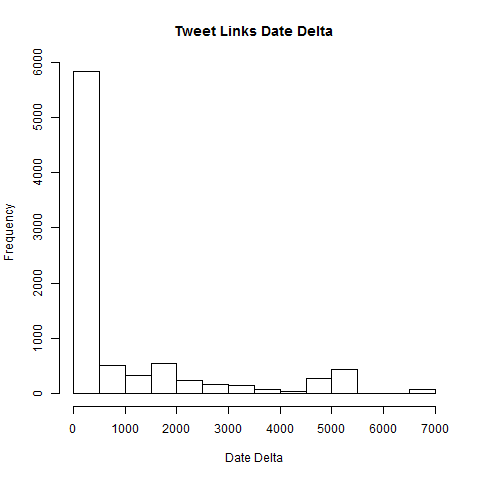
\includegraphics[scale=0.60]{tweet-link-age-histogram.png}
        \caption{Delta between the Tweet and URI dates and their number of occurrences}
        \label{Delta between the Tweet and URI dates and their number of occurrences}
    \end{center}
\end{figure}

\subsubsection{tweet-link-age-histogram.R}
\lstinputlisting[language=R,breaklines = true,frame=single,caption={R program to plot the histogram for Tweet and URI dates}, label=lst:q2R,captionpos=b,numbers=left,showspaces=false,showstringspaces=false,basicstyle=\footnotesize]{tweet-link-age-histogram.R}


\subsection{Summary of Tweet and URI's date delta}
\begingroup
\obeylines
\input{summary.txt}
\endgroup
